\documentclass[a4paper,10pt]{article}
\usepackage[utf8]{inputenc}
\usepackage{graphicx}
\usepackage{tipa}

%opening
\title{QCLog}
\author{}

\begin{document}

\maketitle

\begin{abstract}
QCLog is a \textbf{Q}uick, \textbf{C}ontest-oriented amateur radio \textbf{L}ogger.
QCLog prioritizes speed and convenience over features. It's intended
to run reliably and provide a minimal feature set, meeting the essential
requirements for contest logging:

\begin{itemize}
 \item Exchange logging (callsign/class/section by default, but customizable)
 \item Dupe checking
 \item Band/mode synchronization from the rig
 \item Current operator
 \item Network sync between multiple logging stations
\end{itemize}

Other features --- common in (contest) loggers --- are excluded to eliminate dependencies,
simplify the UI, and avoid annoying behavior like unreadable text in dark-mode desktop themes.

\end{abstract}

\tableofcontents

\section{Logging with QCLog}
The QCLog exchange field(s) are configurable, but field day is the default and will
be used as an example throughout this guide. See Figure \ref{fig:main} for the basic QCLog interface.

\begin{figure}[!htb]

\centerline{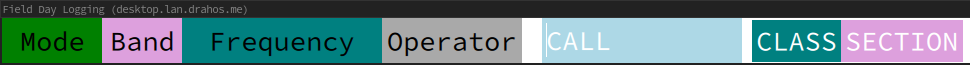
\includegraphics[scale=0.5]{main.png}}
 
\caption{QCLog interface}
\label{fig:main}
\end{figure} 

The main focus of the QCLog UI is to be simple and consistent. To wit:
\begin{itemize}
 \item Escape \emph{always} clears all input and returns the cursor to callsign input.
 \item Tab cycles through input fields in order (callsign/class/section).
 \item Enter submits a log entry, rejecting duplicate or incomplete entries
 \item Ctrl-enter force logs \emph{whatever} is currently entered, no matter what.
 \item The Mode/Band/Frequency/Operator fields are set by right-clicking to spawn a dialog.
 Note that Mode/Band/Frequency will be auto-populated by appropriate rig integration, but
 operator must be manually set (or specified by command line options at startup).
\end{itemize}

\begin{figure}[!htb]
 \centerline{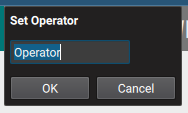
\includegraphics{operator.png}}
 \caption{``Set Operator'' dialog when right-clicking on ``Operator'' field}
 \label{fig:operator}
\end{figure}

See Figure \ref{fig:operator} for the ``Set Operator'' dialog. Depending on
window manager behavior, the full dialog might not appear (see the documented \textbf{BUG}).

\begin{figure}[!htb]

\centerline{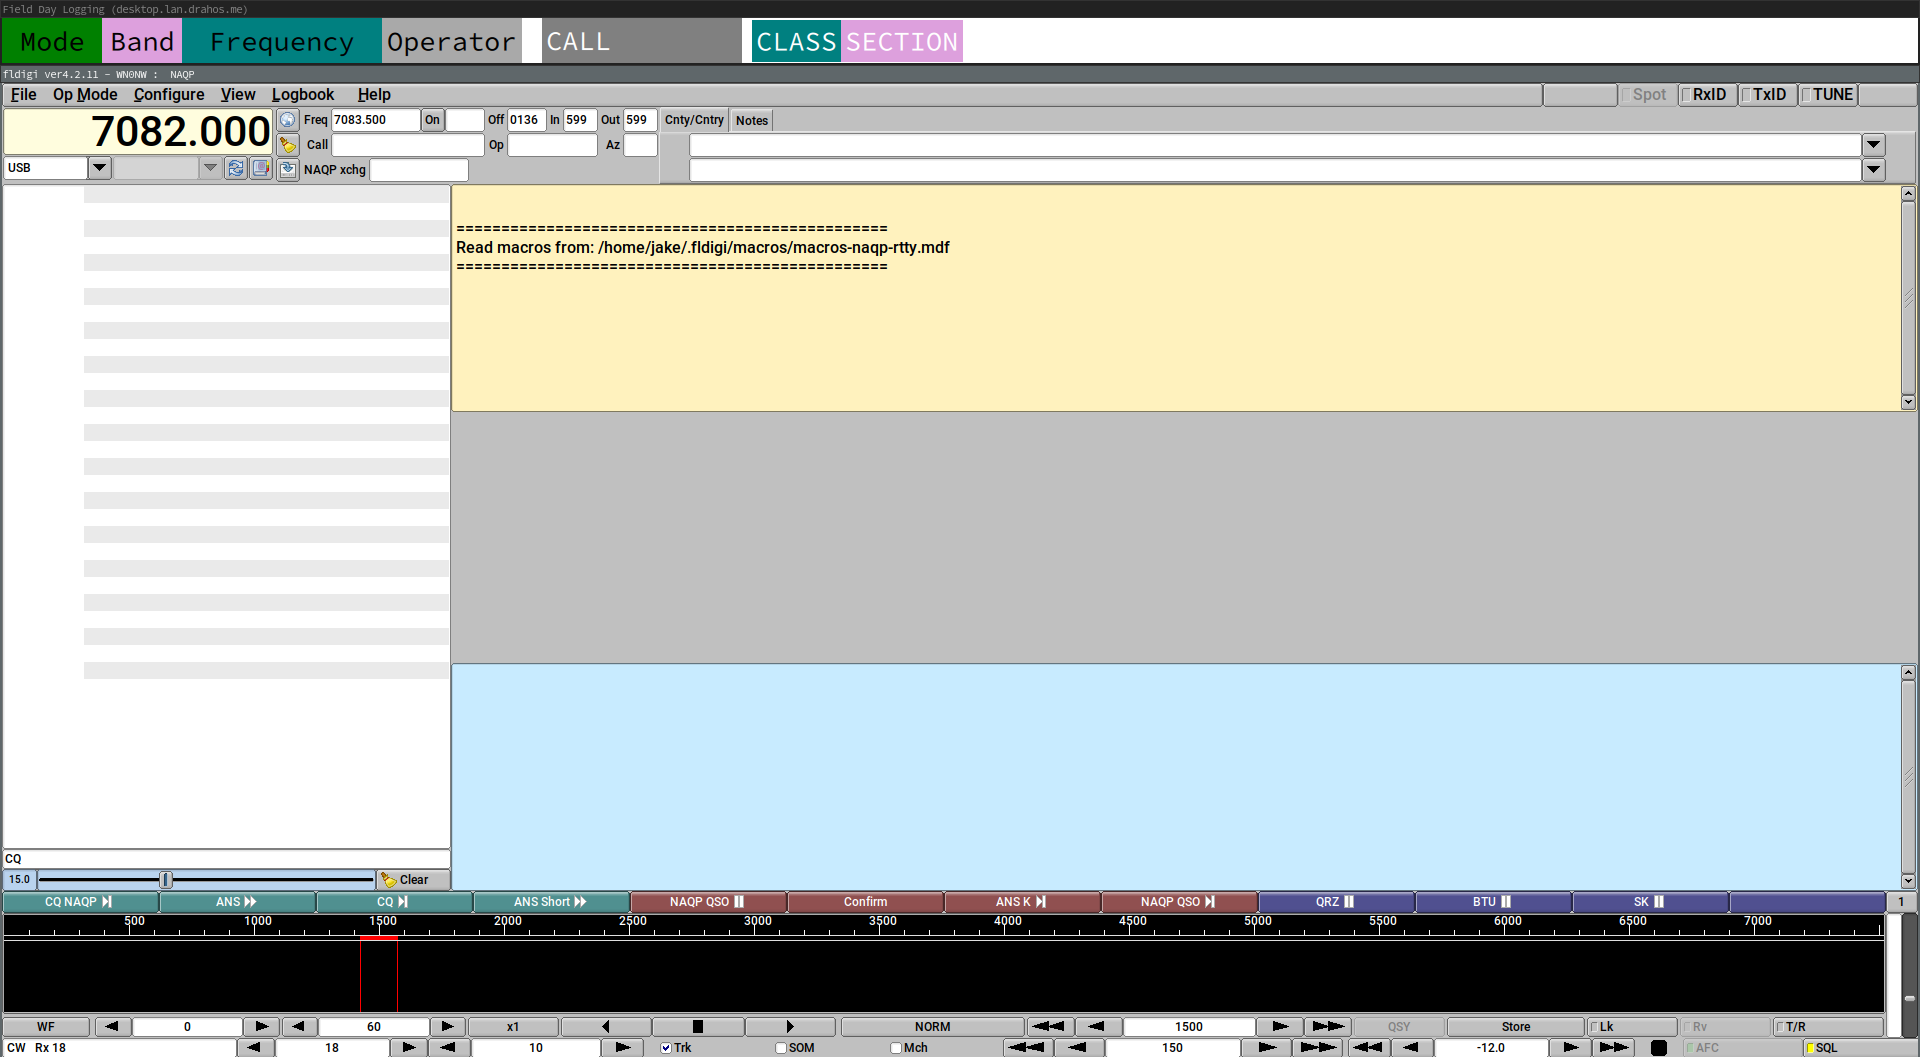
\includegraphics[scale=0.3]{fldigi.png}}
\caption{QCLog tiled with FLDigi}
\label{fig:tile}
\end{figure}

While a tiling window manager is not required, QCLog is intended to cooperate
very well with a tiling window manager (or tiling features of another type of
window manager). Figure \ref{fig:tile} shows QCLog tiled with FLDigi (a major intended use-case).

The intent is that it will look and feel like a native extension of any other program
that might be in use at the time. QCLogs is to accept log entries, flag dupes, and that's all.

\textbf{BUG:} QCLog doesn't currently supply the right window hints to fully float
the dialog when right clicking to edit a field, so the dialog is bounded to the height of
the QCLog main window in i3. The field won't be visible, but it still gets keyboard focus,
so operator etc. can be manually input.

\textbf{A note on modifying/deleting entries.} You can't. But, you can always
just type ``DELETE THE PREVIOUS QSO'' or ``PREV SECTION SHOULD BE IL'' into
the callsign field, then ctrl-enter to force log it. Clean it up after exporting
Cabrillo; it should be easy to catch since such ``notes'' will pretty obviously 
fail any callsign validation or otherwise stick out like a sore thumb.

\subsection{Status}

\begin{figure}[!htb]
 \centerline{
\includegraphics[scale=0.8]{status.png}}
 \caption{Status bar of QCLog}
 \label{fig:status}
\end{figure}

The title bar provides log confirmation and basic status. Refer to Figure \ref{fig:status}.
The status items are:
\begin{itemize}
 \item ``Field Day Logging'' --- Name taken from interface definition.
 \item ``(desktop.lan.drahos.me)'' --- Station name. Defaults to hostname, but can be overridden with
 command line options (see Networking for more details).
 \item ``Logged KF0TEST at 03:59:07UTC'' --- Log confirmation (most recent local QSO).
 \item ``KE0CDT logged by chromebook at 05:42:16UTC'' --- Most recent remote log (logging station ``chromebook''
 logged callsign ``KE0CDT'').
\end{itemize}

\begin{figure}[!htb]
 \centerline{
\includegraphics[scale=1.0]{rigerror.png}}
 \caption{Important status message (rig communication lost)}
 \label{fig:error}
\end{figure}

The status in the title bar largely provides confirmation. Important alerts show up in red to the
right of the exchange entry, as shown in Figure \ref{fig:error}

\subsection{Advanced Usage}
Logs are stored in a SQLite database. The schema is somewhat flexible for the exchange, 
but callsign/timestamp and meta-information (band/mode/freq/operator) are required.
All QSOs are assigned a UUID when logged, which is used for network synchronization and
deduplication. Logs are stored in \texttt{\$XDG\_DATA\_HOME/qclog/<log name>.db} (Default 
\texttt{.local/share/qclog/<log name>.db}).

The database schema isn't the simplest thing, but the \texttt{log} view
contains everything you might need for manual log surgery or export (see
Figure \ref{fig:query} for an example of directly querying the log). If you're brave enough
to try modifying the underlying logs, the tables are \texttt{qsos} and
\texttt{remote\_qsos}. The \texttt{log} view is mostly sort of a deduplicated
concatenation of these two underlying tables. I usually just wait until after
Cabrillo export to clean things up in a text editor.

\begin{figure}[!htb]
\centerline{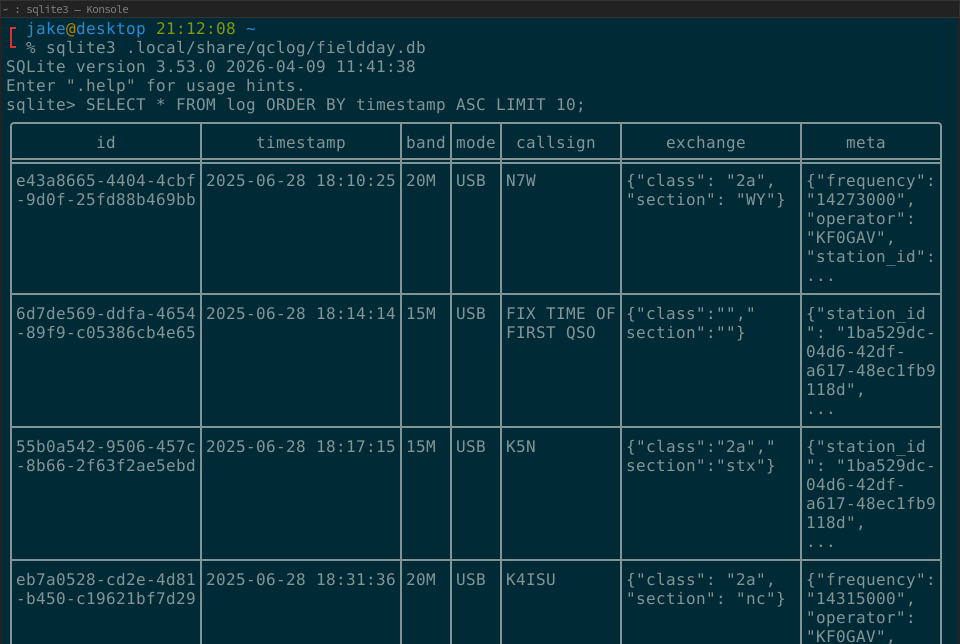
\includegraphics[scale=0.6]{db.png}}
 \caption{Querying the log}
 \label{fig:query}
\end{figure}

QCLog also stores ``disaster logs'' which are append-only and always flushed. A new file is
created timestamped at each start and log a plain-text version of the log entry. Should 
something horrible happen to the SQLite database, you should be able to reconstruct the
log from the disaster logs. The disaster logs are stored in the same directory as the database
files.

There isn't currently any functionality to actually import a disaster log, but all the data is there.
Actually recovering from database corruption or similar disaster is left as an exercise to the reader.

For hints on further log manipulation,
see the SQLite documentation, particularly for JSON operations.

\subsection{Networking}
Networking mostly just works\textsuperscript{\texttrademark}. QCLog uses UDP broadcasts
on port 14300. If you have a system-level firewall, make sure 14300/udp is open since there
isn't any \texttt{connected/established} state with UDP to make default firewall rules happy.
Especially with broadcast UDP.

QCLog networking uses UUIDs to identify different logging stations (operating positions). The
station UUID is stored in the database and generated the first time QCLog is launched
for a given log name. Additionally, the \texttt{-n <station name>} command line parameter
can be used to set a station name overriding the hostname. Any station name specified with
\texttt{-n} is cached in the database and will be used even if no \texttt{-n} parameter
is supplied on subsequent runs (for a given log name). This should help prevent
accidentally reverting the station name to the hostname.

\subsubsection{Resync and Network Traffic}
QCLog is fairly reasonable when it comes to network traffic. QSOs are broadcast when logged
(several hundred bytes at most) and acknowledged when received (several dozen bytes). Stations
periodically heartbeat, which includes the station UUID, station name, and local QSO count.

A resync can be triggered if a station realizes it is ``missing'' QSOs. The
resync algorithm is rather primitive, but should scale okay for reasonable QSO counts. Transfers
are chunked, so even if a link gets saturated and packets drop, there will still be progress
with the resync and the next resync period should start further along.

Overall, QCLog networking seems to work well and be stable on any reasonable WLAN. However,
it is \emph{highly} inadvisable to try to run it over a 1200-baud packet link or similar
silliness. Attempting to do so would almost certainly lead to interesting results.

\section{Command Line}
The only mandatory argument is the ``log name''. Saved settings (and, of course, log entries)
are stored under this name. Field Day is the default exchange interface.

\texttt{--help} is fully implemented. 

\subsection{ADIF export for POTA}
ADIF export is basically a prototype for POTA. Simply supply \texttt{MYCALL:MYPARK} and a
mostly POTA-compatible ADIF will probably be exported. See \texttt{--help} and \texttt{--adif}.

\subsection{Cabrillo export}
Oh boy this is hacky. There's a raw Python script in
the QCLog directory that seems to work. The invocation is somewhat arcane, but Figure \ref{fig:cabrillo}
is an example of field day Cabrillo export.

Basically, the argument to \texttt{-c} is a template for
each Cabrillo line. Eache ``word'' in the space-separated list
is a Cabrillo column, and must contain a colon (``:'') followed
by the column width (Cabrillo is technically a fixed-width format). Column templates
are literal, unless matching one of the templates. \texttt{\%C} is 
replaced with the callsign, while \texttt{\%M} and \texttt{\%E} populate
from the metadata and exchange, respectively. The echange and meta templates
are immediately followed by the name of the JSON field to extract. Of course,
all template arguments must include the width specifier.

\begin{figure}[!htb]
\centerline{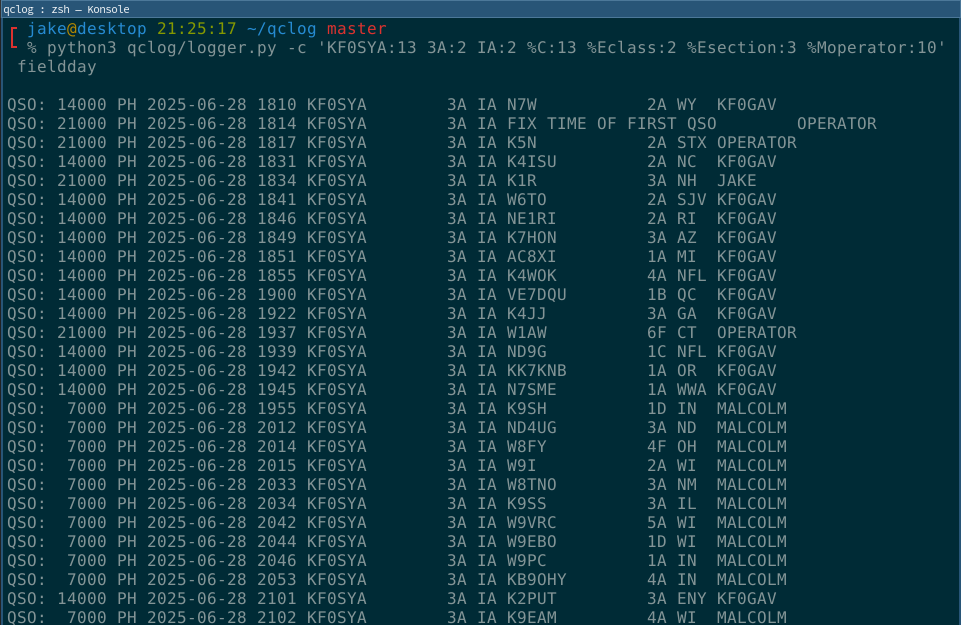
\includegraphics[scale=0.6]{export.png}}
\caption{Exporting Cabrillo}
\label{fig:cabrillo}
\end{figure}


Knowing this, the example in Figure \ref{fig:cabrillo} breaks down to:
\begin{itemize}
 \item \texttt{KF0SYA:13} --- Our callsign (literal)
 \item \texttt{3A:2} and \texttt{IA:2} --- Our exchange (literal)
 \item \texttt{\%C:13} --- Logged callsign
 \item \texttt{\%Eclass:2} --- ``class'' field from exchange JSON
 \item \texttt{\%Esection:3} --- ``section'' field from exchange JSON
 \item \texttt{\%Moperator:10} --- ``operator'' field from metadata JSON
 \item \texttt{fieldday} --- Log name (not part of the \texttt{-c} argument)
\end{itemize}

\section{Common Setups}
\subsection{Standalone}
Of course, it's completely possible to use QCLog without any rig integration.
Band/mode/frequency can be initially populated with command-line flags and changed
at runtime by right-clicking on the field.

This is not recommended for obvious reasons. Sorting out 3 hours of logging
under the wrong band/mode at 8am on field day sunday is a headache.

\subsection{Digital Modes (Full FLDigi integration)}
\textbf{TL;DR:} If you already have working, mostly-default FLDigi, just run with \texttt{--fldigi} 
and \texttt{--flrig} to enable the FLDigi integration and get band/mode from FLRig. 

When running FLDigi with mostly-default rig control settings
settings, FLRig takes full control of the rig. Both FLDigi and FLRig have
partially-documented XMLRPC interfaces. QCLog
will query FLRig for rig data to populate band/mode/frequency. The FLDigi integration
simply auto-populates QCLog with any callsign selected in FLDigi. Before starting QCLog,
start FLDigi and configure it to use FLRig (either by manually starting FLRig before
FLDigi or doing whatever magic lets FLDigi run/manage its own FLRig instance).

Figure \ref{fig:fldupe} shows an example of the FLDigi integration. When
you click on a callsign in the FLDigi text windows, it will populate
FLDigi's callsign logging field. QCLog monitors that field over
the XMLRPC interface (when running with \texttt{--fldigi}), and will auto-populate
its callsign input. This will trigger a dupe warning as appropriate.

\begin{figure}[!htb]
 \centerline{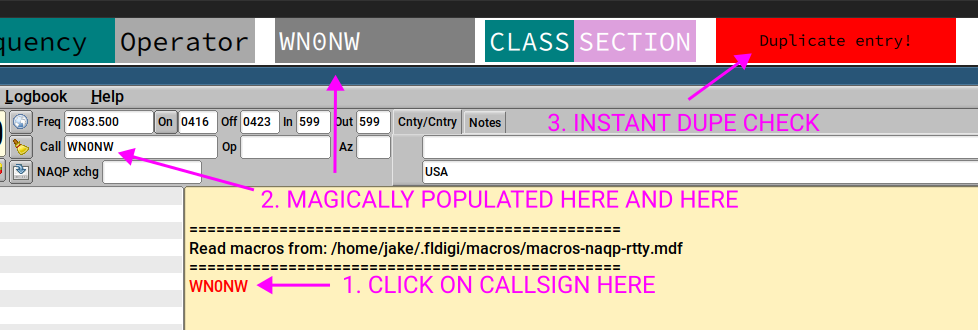
\includegraphics[scale=0.6]{fldigi2.png}}
 \caption{Dupe checking with FLDigi integration}
 \label{fig:fldupe}
\end{figure}

FLRig integration is enabled with \texttt{--flrig} and FLDigi with \texttt{--fldigi}.
There are no arguments for either option, since FL(Rig\textpipe Digi) always use
the same port for XMLRPC.

\subsection{FLRig-only}
FLRig can be run independetly of FLDigi. If you can figure out how to run
with \texttt{--fldigi} and \texttt{--flrig}, you can probably figure out
how to use only \texttt{--flrig}.

\subsection{Rigctld}
FLRig can sometimes be not-so-stable, or you might not have any FL.* installed.
\texttt{rigctld} is installed as part of Hamlib and accepts the same arguments as
\texttt{rigctl}, plus specifying a TCP port to listen on. Simply start 
\texttt{rigctld} before QCLog with all other necessary arguments, then
run QCLog with \texttt{--rigctld <rigctld listen port>}.

\subsection{Hamlib (TERRIBLE)}
\textbf{DO NOT USE. HORRIBLY HORRIBLY BROKEN}. Hamlib has a habit of
killing the whole process when there are errors. Will probably replace Hamlib
with a popen'd rigctl or something.

\section{Installation and Dependencies}
QCLog is a minimal-dependency Python/Qt6 application. The only dependencies are:
\begin{itemize}
 \item Qt6 + PySide6
 \item Python SQLite and XMLRPC
\end{itemize}

The SQLite and XMLRPC modules are part of the Python standard libraries, so if
you have Python, you should \emph{really} have those. Note that the database schema
does use some SQLite JSON operators which require a relatively recent version
of SQLite3. A certain distribution apparently decided to ship a circa-2019 version of SQLite3
for their 2022 LTS release in the year of our Lord 2025 for some inconceivable reason.
This caused problems at field day.

PySide6 is the official Qt binding for Python. Practically all distributions ship
it in the repositories. \texttt{.deb}-based distributions might not pull in all QPA
dependencies when installing PySide6, so unless you already have a good number of
Qt or KDE applications/DE, you might get fun errors. \texttt{libxcb} really likes
to cause problems. It should also be noted that frankendebians are \emph{really} bad
at shipping a working distribution of PySide6.

No issues have been observed on OpenSUSE:

\begin{verbatim}
 # zypper in python313-pyside6
\end{verbatim}

Will install the only actual dependency of QCLog. Then it just works\textsuperscript{\texttrademark}.

Obviously, FL(Digi\textpipe Rig) or rigctld need to be installed if you want to use those
features.

There's no real versioning and absolutely no promise of network interoperability between
different commits. To install, simply acquire via git:

\begin{verbatim}
 $ git clone https://github.com/drahosj/qclog
\end{verbatim}

With the dependencies installed, it should just...run.

\begin{verbatim}
$ qclog/main.py logname
\end{verbatim}

You can also be cool and set up an alias/symlink/whatever floats your goat. Everything should be
relative to the entry point script location, so you don't need to \texttt{cd} into the
\texttt{qclog} directory first.

\subsection{Flatpak}
It turns out that QCLog builds and runs perfectly well as a flatpak. With the ``networking'' permission,
XMLRPC integration, networking, and rigctld integration all work. Logs are stored in the modified
\texttt{\$XDG\_DATA\_HOME} per the Flatpak specification.

Actually doing so is left as an exercise for the reader.

\subsection{Windows}
lol

\section{Extending}
The front-end is written in QML. The \texttt{Interfaces} directory contains the top-level
files, which are used to configure the exchange. Look at the existing examples.

The interface can be selected with \texttt{-i <interface>} when starting QCLog.

\section{The Future}
QCLog will not see major further development. It worked for a field day, and that's all
that matters. This documentation could quite likely be the final commit.

However, a QCLog-ng is in the works. QCLog-ng will keep the same frontend, but
otherwise be a C++ rewrite of the logger core for better maintainability and
further reduced dependencies.
\end{document}
